\documentclass[a4paper]{article}

\usepackage[portuguese]{babel}
\usepackage{comment}
\usepackage[T1]{fontenc}
\usepackage[utf8]{inputenc}
\usepackage{hyperref}
\usepackage{graphicx}
\usepackage{float}
\usepackage{multirow}
\usepackage[hypcap]{caption} % makes \ref point to top of figures and tables

\begin{document}

\begin{titlepage}

\begin{center}


\includegraphics[width=6cm]{./title}\\[3cm]

\textsc{\LARGE Projecto de Sistemas Digitais}\\[1.5cm]

\textsc{\Large Laboratório 2}\\[1.5cm]


{ \huge \bfseries Escalonamento e Partilha de Recursos \\[3cm] }


\noindent
\begin{minipage}{0.4\textwidth}
\begin{flushleft} \large
Rafael Gonçalves, 73786
\end{flushleft}
\end{minipage}
\begin{minipage}{0.4\textwidth}
\begin{flushright} \large
Gonçalo Ribeiro, 73294
\end{flushright}
\end{minipage}

\vfill

{\large \today}


\end{center}

\end{titlepage}

\tableofcontents
\pagebreak

\section{Arquitectura}
\subsection{Descrição}
A arquitectura que decidimos implementar divide-se em duas secções distintas, como na maioria das arquitecturas dedicadas:
\begin{itemize}
\item Uma Unidade de Controlo, mais especificamente uma Máquina de Estados
\item Uma Datapath, cuja especificação corresponde à disponibilizada no enunciado (ver Figura~\ref{fig:DPdiagram})
\end{itemize}

De modo a melhor fazer a interface com os elementos da placa de desenvolvimento, as várias componentes do sistema foram projectados com vista a fazer a interface com os botões, interruptores e displays da Basys.

Uma vez que da Datapath saem os valores dos registos, que posteriormente terão de ser seleccionados para ir para os displays de sete segmentos, é necessário um multiplexer no exterior da mesma, cujo sinal de selecção provém dos interruptores da placa de desenvolvimento.

\pagebreak
\subsection{Esquemas}
\begin{figure}[H]
	\centering
	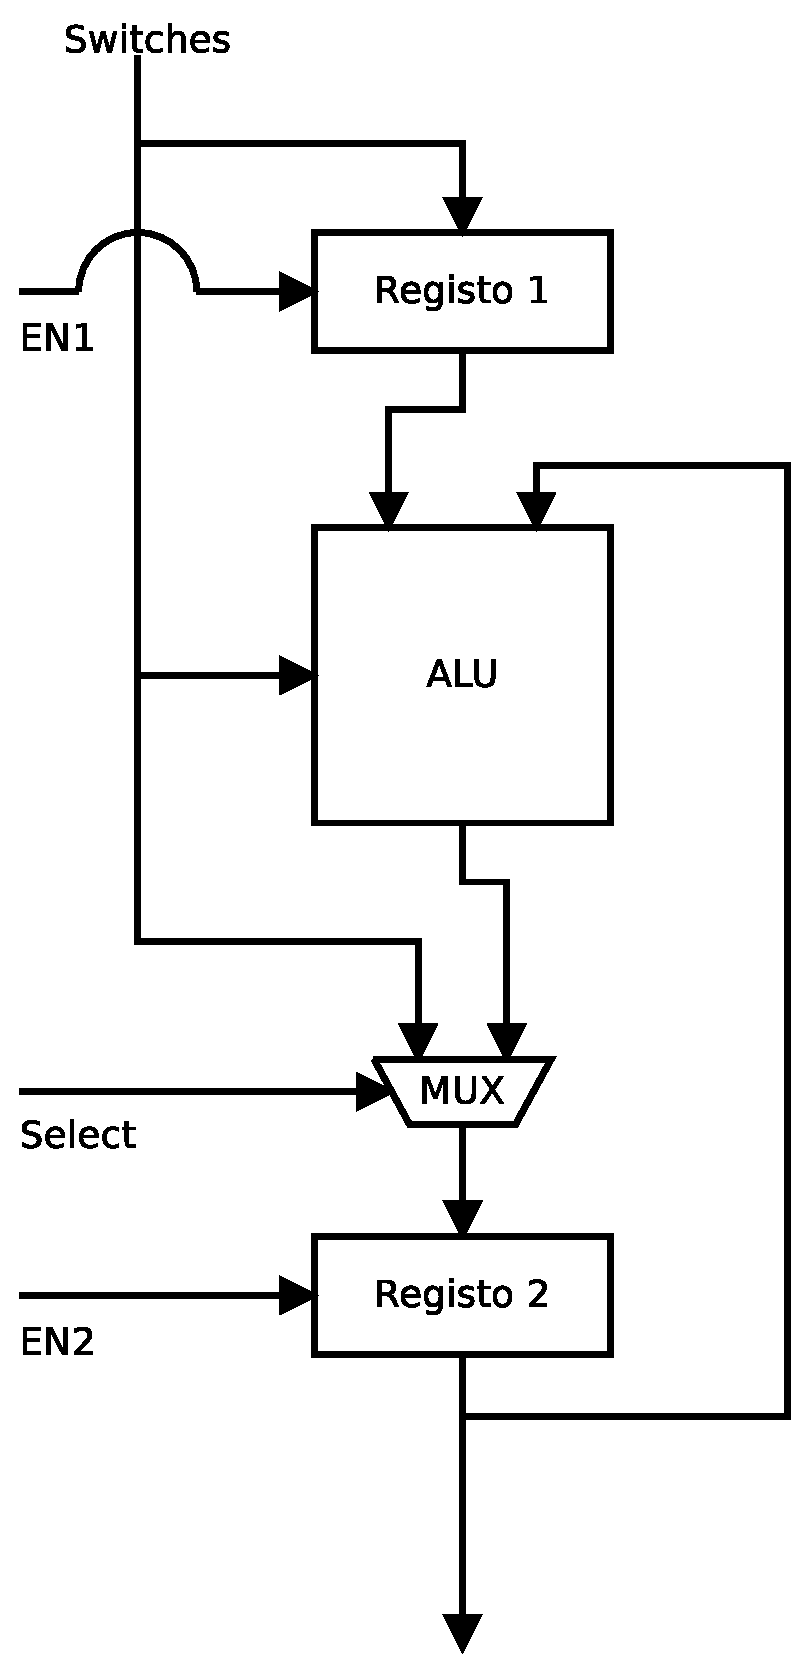
\includegraphics[scale=0.28]{DP}
	\caption{Datapath}
	\label{fig:DPdiagram}
\end{figure}
\begin{figure}[H]
	\centering
	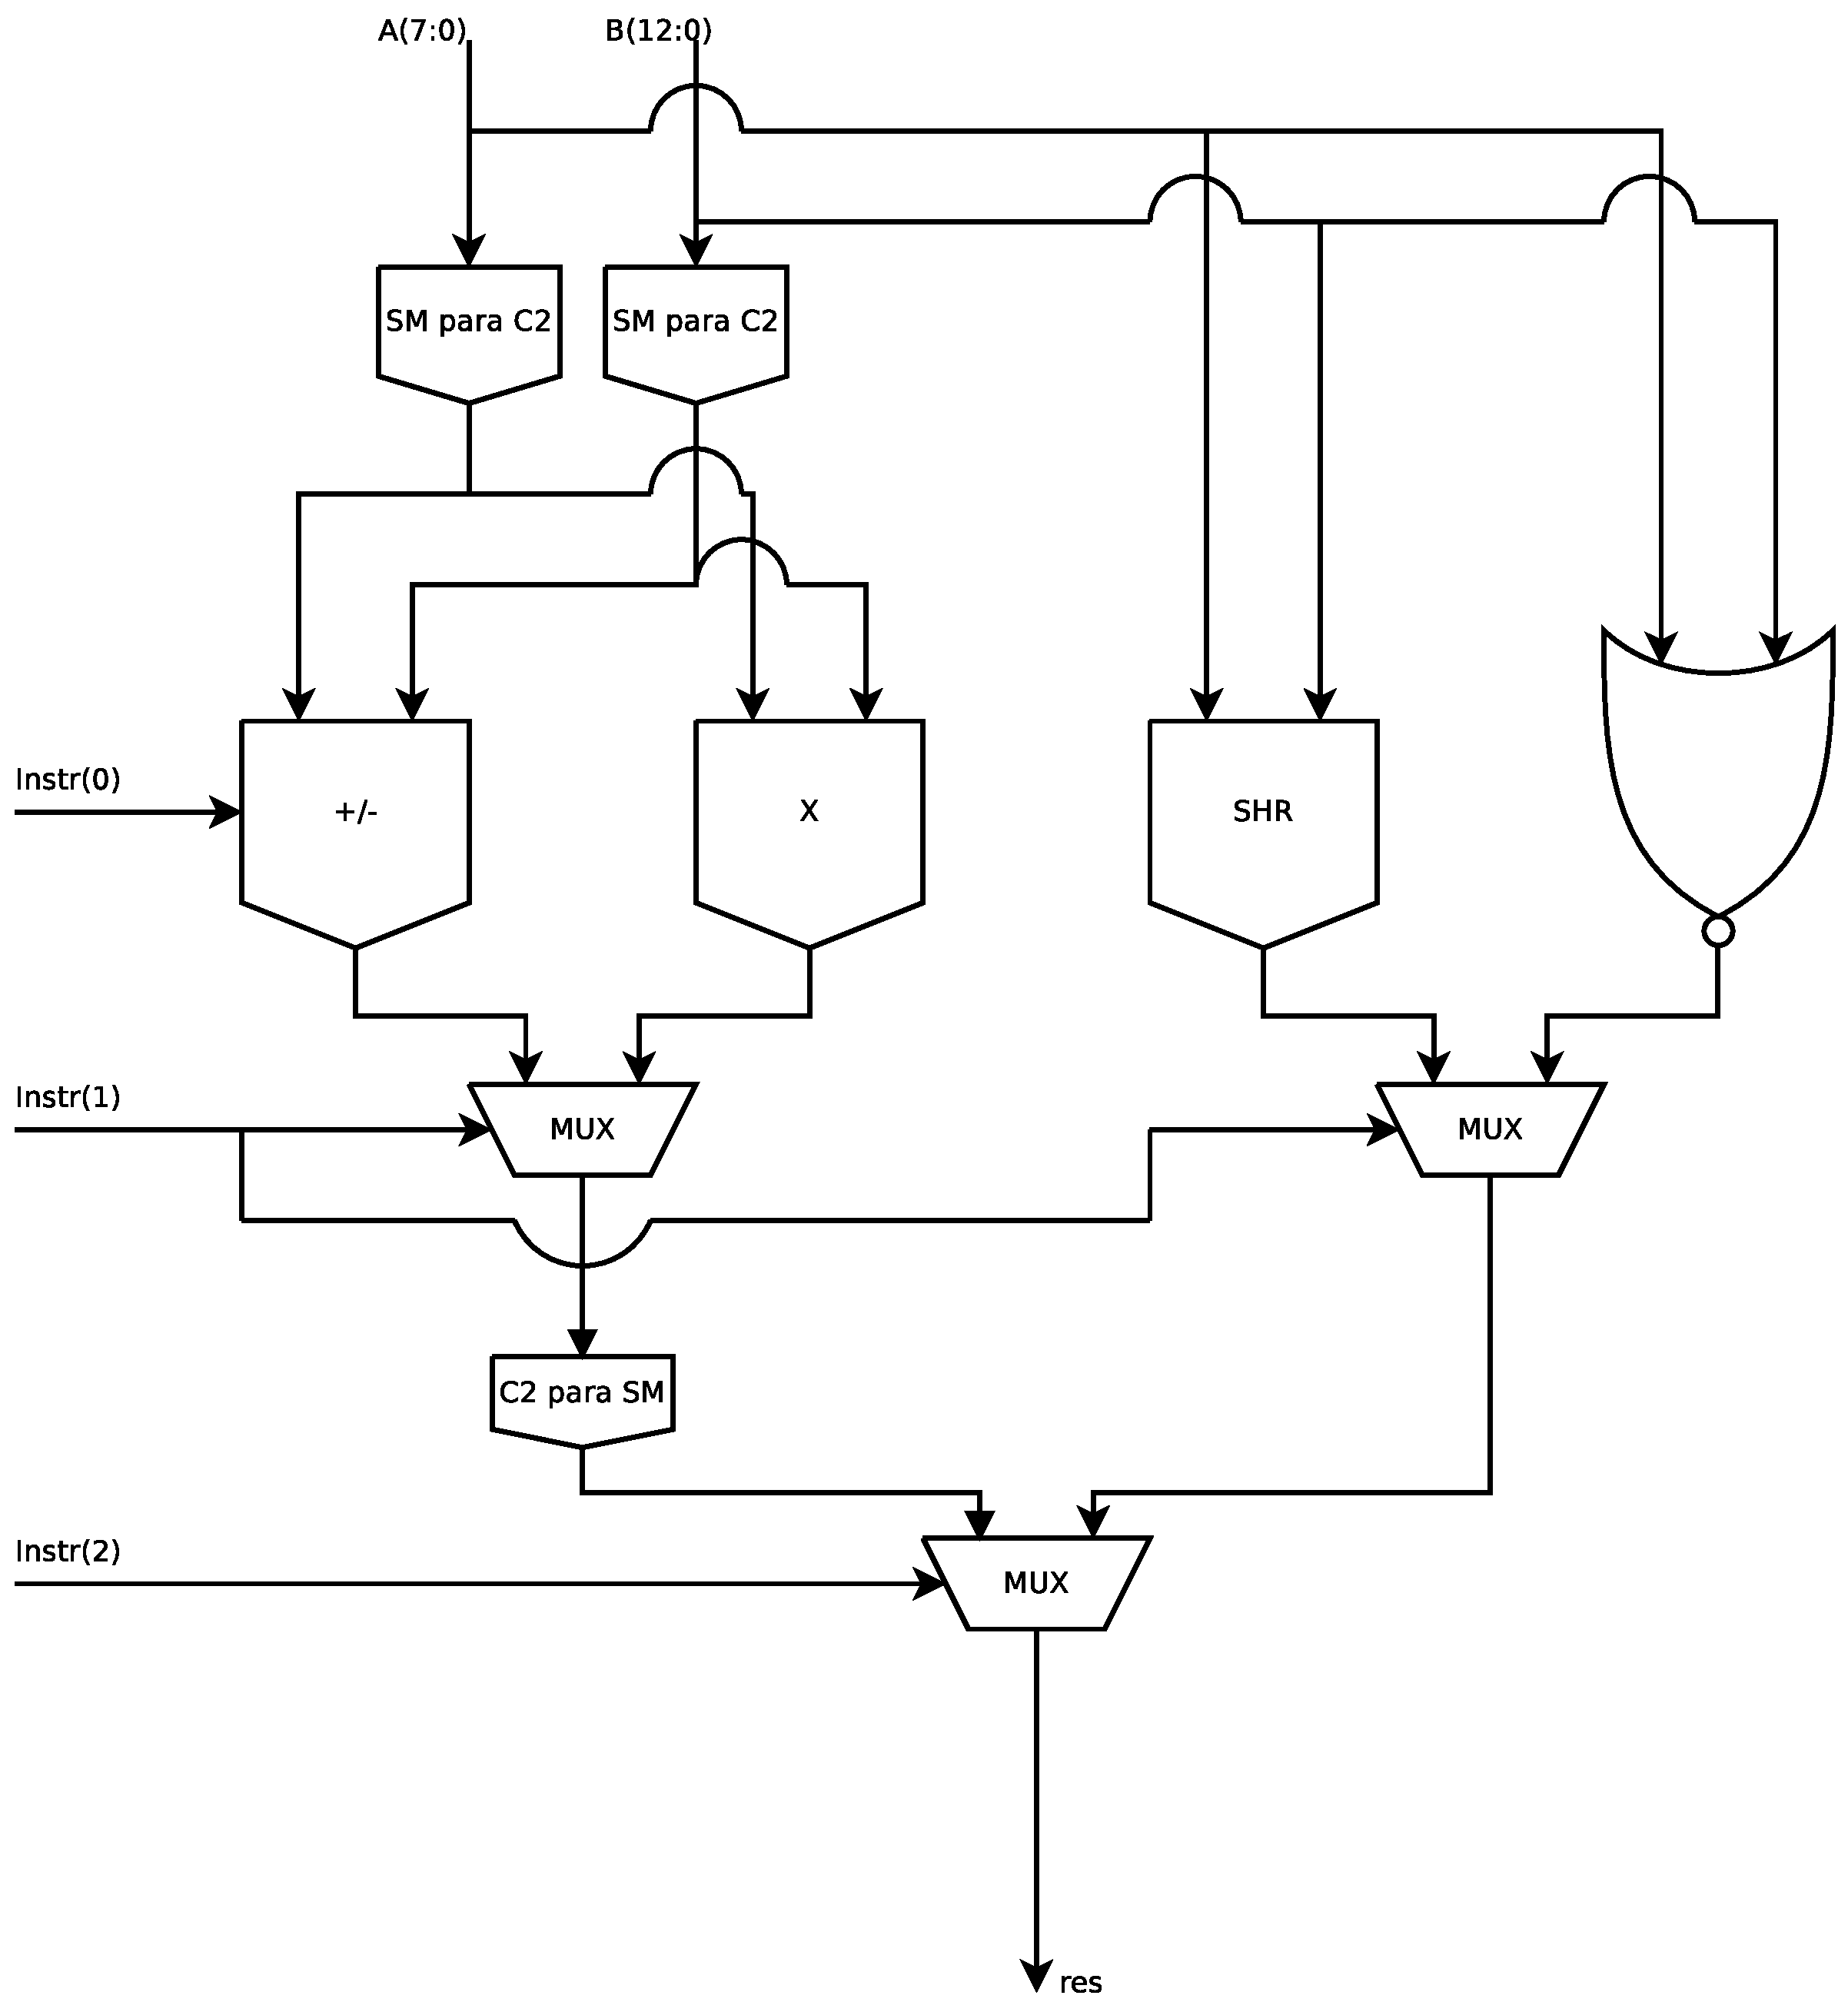
\includegraphics[scale=0.28]{ALU}
	\caption{Unidade Lógico-Aritmética}
	\label{fig:ALUdiagram}
\end{figure}
\pagebreak

\section{Datapath}
\subsection{Descrição}
A decisão mais relevante na datapath foi a codificação de sinal utilizada nos registos e na Unidade Lógico-Aritmética.

De modo a compreender intuitivamente os valores em uso, os displays devem mostrar os valores com uma codificação sinal-módulo. Assim, e uma vez que os valores dos displays originam nos registos da Datapath, decidimos que todo o armazenamento de valores deve ser feito em formato sinal-módulo.


\subsection{Registos}
Os registos foram especificados através das funcionalidades de abstracção da linguagem VHDL, isto é, definimos uma arquitectura de registo com número de bits arbitrário. O tamanho de cada instância é depois determinado no código de instanciação.

Neste caso, foram instanciados dois registos, um de 7 bits e outro de 13 bits, consoante a arquitectura especificada no enunciado.


\subsection{Unidade Lógico-Aritmética}
Uma vez que os dois operadores das diversas unidades funcionais que compõem a ULA estão codificados no formato sinal-módulo, é necessário fazer a conversão de sinal-módulo para complemento para dois.

O Somador (que efectua as operações soma e diferença) e o Multiplicador foram incluídos da biblioteca \emph{signed}, pelo que os seus operandos devem ser convertidos em complemento para dois à entrada, e o resultado deve ser convertido para sinal-módulo à saída (ver Figura~\ref{fig:ALUdiagram}).


\subsubsection{Somador}
O Somador efectua uma soma ou diferença, consoante os sinais de controlo, convencional, em complemento para dois.

\subsubsection{Multiplicador}
O multiplicador efectua um produto convencional em complemento para dois. Uma vez que o produto ocupa mais bits que aqueles disponíveis no registo que o deve armazenar, são desprezados vários dos bits mais significativos do resultado.

\subsubsection{Shift Right Aritmético}
A função shift afecta apenas os bits de módulo do valor armazenado no registo 2. O bit de sinal permanece inalterado.

\subsubsection{Função Lógica NOR}
A função lógica NOR aplica-se aos bits de sinal dos dois operadores e aos 6 bits menos significativos dos dois operadores. Os restantes bits do segundo operador (de dimensão 13) são negados (isto é, NOR 0).

\subsubsection{Simulação}
As operações realizadas na simulação são as indicadas na Tabela~\ref{tab:ALUsim}. É de notar que as operações não comutativas são efectuadas na ordem $ Op_2 \cdot \cdot \cdot Op_1 $.
\begin{table}[h]
	\begin{tabular}{|c | c || c | c | c|}
		\hline
		$Op_1$ & $Op_2$ & Operação & Código & Resultado \\
		\hline
		\texttt{-63} & \texttt{4} & \texttt{MUL} & \texttt{01X} & \texttt{-252} \\
		\hline
		\texttt{5} & \texttt{5} & \texttt{ADD} & \texttt{000} & \texttt{10} \\
		\hline
		\texttt{-5} & \texttt{6} & \multirow{2}{*}{\texttt{SUB}} & \multirow{2}{*}{\texttt{001}} & \texttt{11} \\
		\texttt{5} & \texttt{-3} & & & \texttt{-8} \\
		\hline
		\texttt{0bXXX X001} & \texttt{0b0 0000 0000 0111} & \multirow{3}{*}{\texttt{SHR}} & \multirow{3}{*}{\texttt{10X}} & \texttt{0b0 0000 0000 0011} \\
		\texttt{0bXXX X001} & \texttt{0b0 0000 0000 0011} & & & \texttt{0b0 0000 0000 0001} \\
		\texttt{0bXXX X010} & \texttt{0b0 0000 0000 1111} & & & \texttt{0b0 0000 0000 0011} \\
		\hline
		\texttt{0b000 0001} & \texttt{0b0 0000 0000 0010} & \texttt{NOR} & \texttt{11X} & \texttt{0b1 1111 1111 1100} \\
		\hline
		\texttt{5} & \texttt{127} & \multirow{3}{*}{\texttt{MUL}} & \multirow{2}{*}{\texttt{01X}} & \texttt{635} \\
		\texttt{63} & \texttt{4095} & & & \texttt{4033} \\
		\texttt{-63} & \texttt{4095} & & & \texttt{-4033} \\
		\hline
	\end{tabular}
	\caption{Operações da Simulação da Figura~\ref{fig:ALUsim}}
        \label{tab:ALUsim}
\end{table}

\begin{figure}[h]
	\centering
	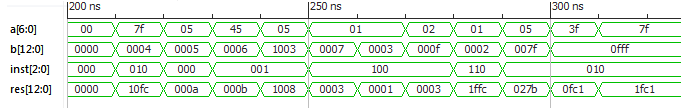
\includegraphics[width=\textwidth]{ALU_sim}
	\caption{Simulação da Unidade Lógico-Aritmética}
	\label{fig:ALUsim}
\end{figure}
\pagebreak


\section{Unidade de Controlo}
\subsection{Descrição}
A Unidade de Controlo implementa a Máquina de Estados e é o componente responsável por controlar os multiplexers e os enables e sinais de reset dos registos da Datapath. Como input tem os sinais da FPGA que permitem escolher a operação a realizar.

\subsection{Máquina de Estados}
A Máquina de Estados implementada é a da Figura~\ref{fig:FSMdiagram}. Tem um estado inicial e um final, dois estados de load e um de operação.

Nos estados \textit{load1} e \textit{load2} o valor à entrada da datapath é armazenado nos registo correspondente. No estado \textit{op} o resultado da ULA é armazendo no registo R2. A operação que a ULA deve realizar é controlada pelo utilizador sob a forma do sinal INST à entrada da datapath.

\begin{figure}[h]
	\centering
	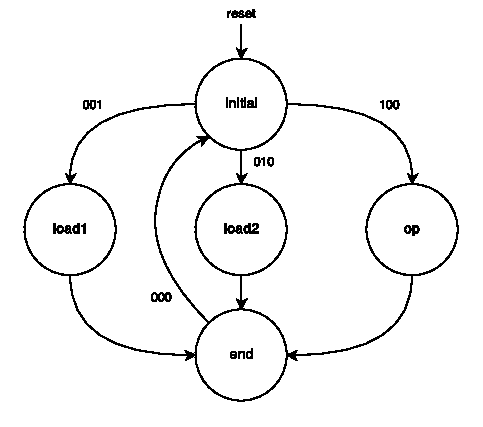
\includegraphics[scale=0.28]{FSM}
	\caption{Máquina de Estados}
	\label{fig:FSMdiagram}
\end{figure}

\subsection{Sinais de Controlo}
Os sinais que entram na Datapath vindos da Unidade de Controlo são três: dois sinais controlam a escrita nos registos R1 e R2; um outro sinal controla o multiplexer que existe antes de R2.

No estado \textit{load1} o enable de R1 é posto a high. No estado \textit{load2} o enable de R2 fica a high e o multiplexer deixa passar o valor à entrada da datapath.

Por fim no estado \textit{op} o enable de R2 é posto a high e o multiplexer deixa passar o sinal à saída da ULA.

\subsection{Simulação}
A simulação da Unidade de Controlo pode ser vista na Figura~\ref{fig:controlo_sim}. Nesta simulação pode verificar-se que a sequência de estados corresponde à descrita na Figura~\ref{fig:FSMdiagram} e que os sinais de controlo estão correctos.

\begin{figure}[H]
	\centering
	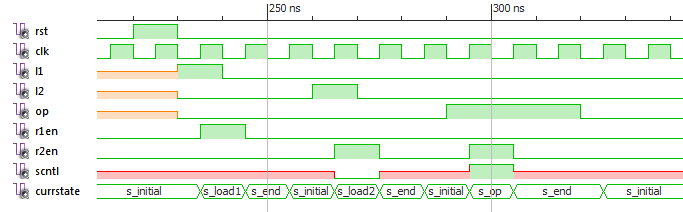
\includegraphics[width=\textwidth]{control_sim}
	\caption{Simulação da Unidade de Controlo}
	\label{fig:controlo_sim}
\end{figure}

\pagebreak


\section{Simulações}
A simulação que verifica o correcto funcionamento dos diversos elementos em conjunção pode ser vista na Figura~\ref{fig:circuit_sim}. São realizadas algumas operações de significado trivial, com o único propósito de demonstrar a interligação dos diversos blocos. 

\begin{figure}[H]
	\centering
	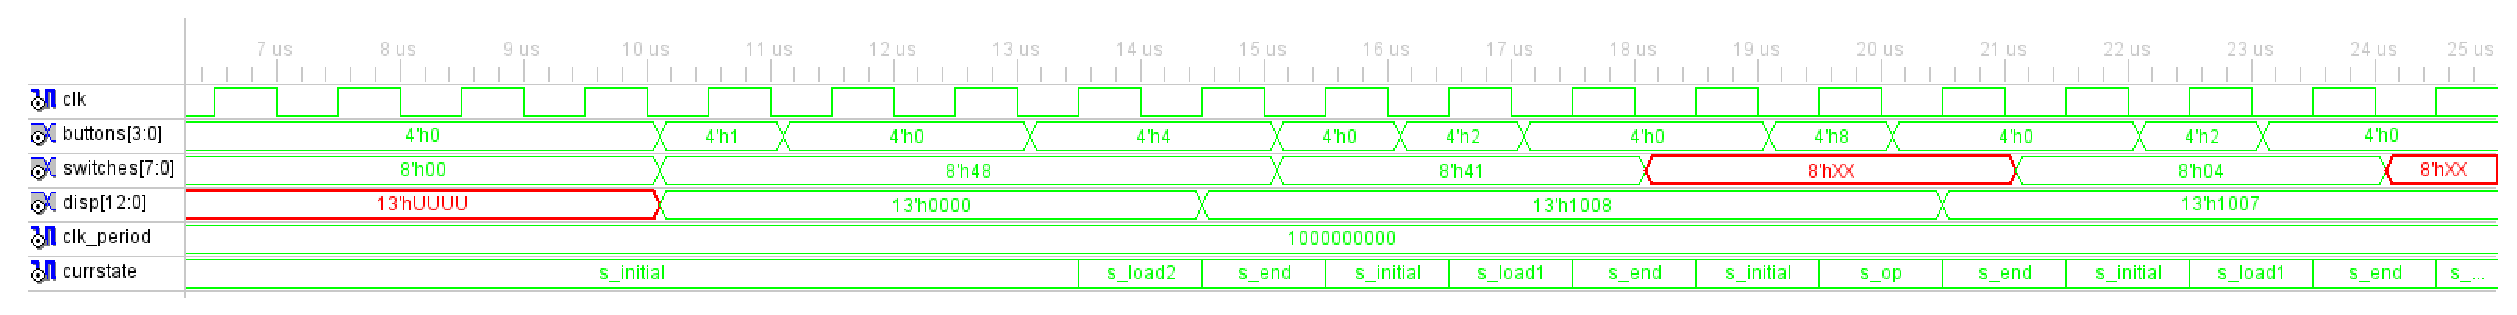
\includegraphics[width=\textwidth]{circuit_sim}
	\caption{Simulação do Circuito Completo}
	\label{fig:circuit_sim}
\end{figure}

\end{document}